\documentclass{TDP005mall}



\newcommand{\version}{Version 0.1}
\author{Hadi Ansari, \url{hadan326@student.liu.se}\\
  Nils Bark, \url{nilba048@student.liu.se}}
\title{Kravspecifikation}
\date{2020-11-17}
\rhead{Hadi Ansari\\
Nils Bark}



\begin{document}
\projectpage
\section{Revisionshistorik}
\begin{table}[!h]
\begin{tabularx}{\linewidth}{|l|X|l|}
\hline
Ver. & Revisionsbeskrivning & Datum \\\hline
0.1 & Första utkastet & 2020-11-17 \\\hline

\end{tabularx}
\end{table}


\section{Spelidé}
Spelet utspelar sig i en 2D-miljö från ett sidoperspektiv. Spelaren kan röra sig i åtta olika riktningar och skjuta skott mot de ankommande fienderna. Skotten som spelaren skjuter gör skada till fienderna den träffar och kommer till slut förstöra den. När en fiende förstörs får spelaren en visst antal poäng. Det finns även en chans att en förstörd fiende släpper ifrån sig en ``Power-up'' som ger spelaren olika fördelar. Det kommer även då och då att dyka upp Power-ups från högra sidan av skärmen. Fienderna kommer att närma sig från höger om skärmen och röra sig mot vänster. Fiendertyperna kan även ha unika rörelsemönster när de färdas över skärmen. Fienderna gör skada till spelaren antigen genom att vidröra den eller genom att träffa spelaren med sina skott (om de skjuter skott). Spelaren har ett antal liv som förloras allt eftersom den har blivit träffad av fienderna/deras skott. När spelarens liv är noll då spelet är slut.

\section{Målgrupp}
Målgruppen är alla som tycker om utmanande skjut-spel i denna klassiska arkad-stil.

\section{Spelupplevelse}
Det roliga med spelet fås från en kombination av den ständigt ökande utmaningen och poänginsamlingen. Spelet kan spelas om och om igen för att få ett så bra poängrekord som möjligt.

\section{Spelmekanik}
Spelaren styrs av W, A, S, D eller piltangenterna. Spelaren skjuter med mellanslag.

\section{Regler}
\subsection{Spelplan}
\begin{itemize}
\item Spelplanen har en fixerad storlek.
\item Spelaren kan endast befinna sig inom spelplanen medan fienderna kan komma in i spelplanen från sidorna. 
\item Objekt som åker ut ur spelplanen förstörs.
\end{itemize}

\subsection{Spelare}
\begin{itemize}
\item Spelaren kan röra på sig i åtta riktningar.
\item Spelaren kan skjuta skott som skadar fienderna när de kolliderar.
\item Spelarens skott minskar fienders liv med 1.
\item Spelaren har en bashastighet som avgör hur snabbt den kan skjuta.
\item Spelaren kan plocka upp Power-ups genom att kolliderar med dem.
\item Spelaren inte kan plocka upp Power-upps genom att förstöra dem med sin skott.
\item Spelaren har tre liv och kan inte gå över detta.
\item Spelaren kan få liv genom att plocka upp heal Power-ups.
\item Spelaren förlorar ett liv när den kolliderar med skot.
\item Spelaren förlorar ett eller två liv när den kolliderar med fiender (beroende på fiendetypen).
\item När spelaren ta skada (kollision med fiende objekt eller deras skott) blir den odödlig i tre sekunder.
\item När spelarens liv är noll förlorar man.


\end{itemize}

\subsection{Fiende}
Fiender i spelet kan inte förtöra varandra med skott eller kollision.
\begin{itemize}
\item Fiender kan röra på sig.
\item Fiender rör sig enligt förbestämda mönster över skärmen.
\item Fiender kan skjuta skott baserat på en timer (till exempel var tredje sekund).
\item Fiender kan skada spelaren genom att kollidera med den.
\item Fiender har också ett antal liv och när de deras liv når noll dör de.
\item Fiender kommer från höger sidan om skärmen och de rör sig år vänster tills de når slutet av sin bana  
\end{itemize}


\subsubsection*{Fiende typ1}
\begin{itemize}
\item Den har ett liv.
\item Den förstörs när den kolliderar med spelaren eller när den träffar spelarens skott.
\item När den kolliderar med spelaren minskar spelarens liv med 1.
\item Dens skott minskar spelarens liv med 1.
\item Den rör sig åt vänster enligt en bestämd vågrörelse (se bild).
\item Den har röreslehastighet 3.
\item Den sjkuter när den är i samma höjd av spelaren med en konstant hastighet (som inte förändras under spelets gång).
\end{itemize}

\subsubsection*{Fiende typ2}
\begin{itemize}
\item Den har två liv.
\item Den förstörs (oavsett om den har ett eller två liv) när den kolliderar med spelaren.
\item Den förstårs när den träffar spelarens skott två gånger.
\item När den kolliderar med spelaren minskar spelarens liv med 2.
\item Dens skott minskar spelarens liv med 1.
\item Den rör sig åt vänster enligt enligt en linjärt mönster (se bild).
\item Röreslehastighet 2.
\item Den sjkuter när den är i samma höjd av spelaren med en konstant hastighet (som inte förändras under spelets gång).
\end{itemize}

\subsubsection*{Bomber}
\begin{itemize}
\item De dycker upp från höger och närmer sig till vänster sidan av skärmen med hastighet 1.
\item Bomber minksar spelarens liv med 1 när de kolliderar med spelaren.
\item De förstörs när de kolliderar med spelaren eller när de kolliderar med spelarens skott.

\end{itemize}

\subsection{Power-up \& föremål}

\begin{itemize}
\item Power-ups kan släppas ifrån fiender när spelaren förstör dem.
\item Power-ups kan också komma in i spelplanen från sidorna.
\item Power-ups kan ge spelaren diverse positiva effekter.
\item Livlådor kan dyka upp antingen från förstörda fiender eller från kanten av skärmen precis som power-ups. De ger spelaren ett liv vid upplockning.
\end{itemize}

\subsubsection{Heal}
\begin{itemize}
\item 
\end{itemize}

\subsubsection{Triple-shot}
\begin{itemize}
\item 
\end{itemize}

\subsubsection{Shield}
\begin{itemize}
\item 10 sek
\end{itemize}


\subsection{Poäng}
\begin{itemize}
\item Att plocka upp Power-ups ger
\item Spelaren får 50 poöng när den förstör en bomb.
\item Fiendetyp 1 ger 100 poäng.
\item Fiendetyp 2 ger 150 poäng. 
\item Spelaren får 300 poäng om den plockar en heal Power-ups när den har redan fullt liv.  
\item Poäng kan samlas genom att förstöra fienderna.

\end{itemize}

\newpage
\section{Visualisering}
Det här är ett exempel på hur spelet kan se ut.


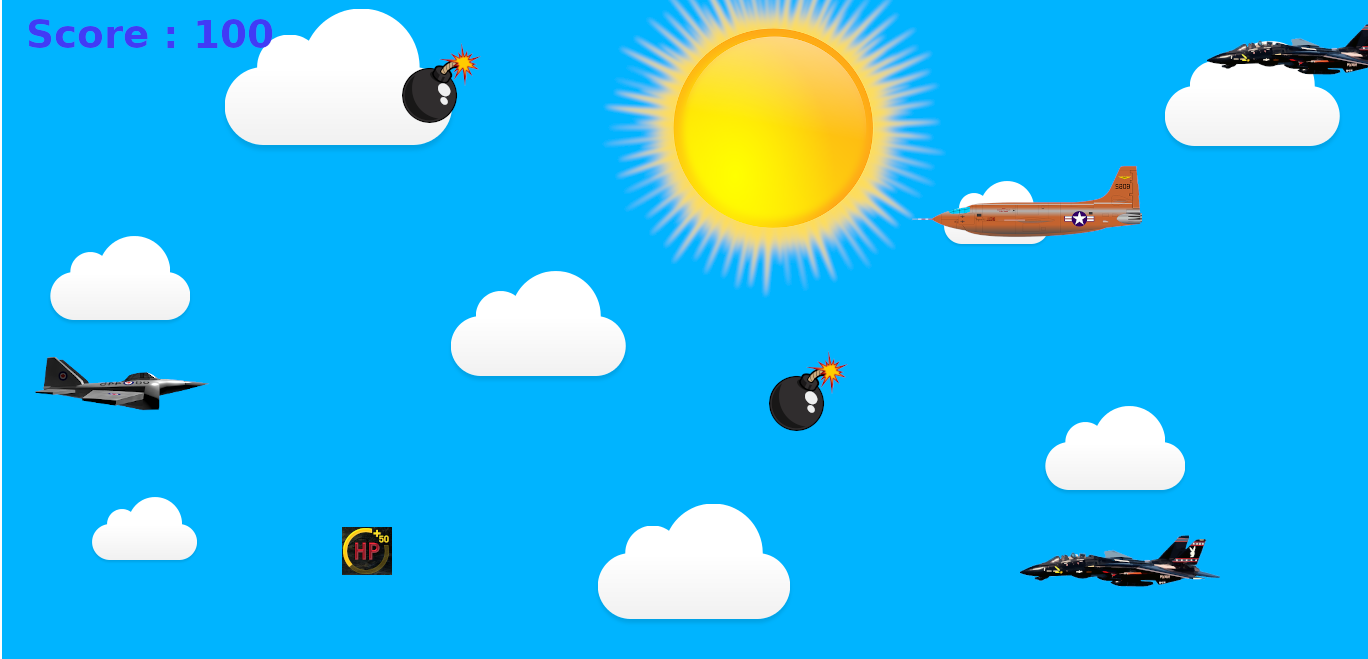
\includegraphics[scale=0.35]{Images/Game.png}

\section{Krav}
\subsection{Ska-krav}
\begin{enumerate}
\item Spelet ska ha en förstasida där en ny runda kan startas, spelet kan avslutas, och eventuella andra sidor kan visas.
\item Spelet ska ha en hjälp-sida där regler och kontroller förklaras.
\item Spelaren ska kunna röra på sig i åtta riktningar som endast begränsas av spelplanens kanter.
\item Spelaren styrs via tangentbordet.
\item Spelaren kan skjuta skott.
\item Spelaren kan förstöra fiender med sina skott.
\item Spelaren kan dö.
\item Spelaren ska tjäna poäng när den förstör ett fiende samt för varje sekund spelaren lever.
\item Spelarens liv och poäng ska konstant visas på skärmen under rundans gång.
\item När spelaren tar skada ska den få en mycket kort period då den ej kan ta skada igen.
\item När spelaren dör ska rundan avslutas och spelaren ges möjlighet att spela igen.
\item Det ska finnas minst två typer av fiender som båda kan röra på sig.
\item Vissa fiender ska skjuta skott.
\item Fiender ska skada spelaren antingen genom att träffa den med skott eller genom att kollidera med den.
\item Fiender ska ha en chans att släppa ifrån sig power-ups när de förstörs av spelaren.
\item Spelet ska öka i svårhetsgrad ju längre spelaren lever. % Hur ska detta ske? Fler fiender? Färre power-ups?
\item Det ska kunna finnas flera fiender av samma typ på spelplanen samtidigt.
\item Spelaren ska kontrollera en spelarkaraktär.
\item Fienderna ska röra på sig enligt ett mönster i spelbanan.
\item Spelet utspelar sig i en 2D-miljö sedd från sidoperspektiv.
\item Spelplanen har en fixerad storlek.
\item Spelaren kan plocka upp Power-ups genom att kollidera med dem.
\end{enumerate}

\subsection{Bör-krav}
\begin{enumerate}
\item Power-ups ska dras mot spelaren då den kommer i närheten av dem
\item Antalet intjänade poäng ska sparas när spelaren till slut förlorar och rundan är avslutad.
\item Spelet ska ha en sida där intjänade poäng från tidigare rundor visas i en topplista.
\item Spelet ska ha en sida där användaren kan ändra vilka tangenter som gör vad.
\item Fiender av samma typ ska kunna ha olika rörelsemönster
\item Spelaren ska förlora poäng när den tar skada. % Kanske på andra sätt också?
\item Det ska finnas svårare versioner av varje fiendetyp som introduceras allt eftersom spelaren överlever en längre tid
\item Bakgrunden ska röra på sig för att ge användaren en känsla av hastighet.
\item Det ska finnas fler rörelsemönster som låter fienderna komma in i spelplanen från andra platser än bara högerkanten.

\end{enumerate}

\section{Kravuppfyllelse}
\textit{\textbf{``Spelet ska simulera en värld som innehåller olika typer av objekt. Objekten ska ha olika beteenden och röra sig i världen och agera på olika sätt när de möter andra objekt.''}}


Uppfylls av krav 3, 4, 5, 6, 12, 13, 14\\


\textit{\textbf{``Det måste finnas minst tre olika typer av objekt och det ska finnas flera instanser av minst två av dessa. T.ex ett spelarobjekt och många instanser av två olika slags fiendeobjekt.''}}


Uppfylls av krav 12, 17, 18\\

\textit{\textbf{``Ett beteende som måste finnas med är att figurerna ska röra sig över skärmen. Rörelsen kan följa ett mönster och/eller vara slumpmässig. Minst ett objekt, utöver spelaren ska ha någon typ av rörelse.''}}


Uppfylls av krav 3, 12, 19\\

\textit{\textbf{``En figur ska styras av spelaren, antingen med tangentbordet eller med musen. Du kan även göra ett spel där man spelar två stycken genom att dela på tangentbordet (varje spelare använder olika tangenter). Då styr man var sin figur.''}}


Uppfylls av krav 3, 4\\

\textit{\textbf{``Grafiken ska vara tvådimensionell.''}}


Uppfylls av krav 20\\

\textit{\textbf{``Världen (spelplanen) kan antas vara lika stor som fönstret ''}}


Uppfylls av krav 21\\

\textit{\textbf{``Det ska finnas kollisionshantering, det vill säga, det ska hända olika saker när objekten möter varandra, de ska påverka varandra på något sätt. T.ex kan ett av objekten tas bort, eller så kan objekten förvandlas på något sätt, eller så kan ett nytt objekt skapas. ''}}


Uppfylls av krav 6, 14, 22\\

\textit{\textbf{``Det ska vara enkelt att lägga till eller ändra banor i spelet. Detta kan exempelvis lösas genom att läsa in banor från en fil, eller genom att ha funktioner i programkoden som bygger upp en datastruktur som definierar en bana.''}}


Vi antar att detta uppfylls av de funktioner vi använder för att få en varierande svårighetsgrad genom att låta fiender röra sig på olika sätt och öka svårighetsgrad. Men vi är osäkra på om detta krav kan uppfyllas på rätt sätt i ett spel som inte har klart definerade banor.\\

\textit{\textbf{`` Spelet måste upplevas som ett sammanhängande spel som går att spela! ''}}

Ska uppfyllas av alla ska-krav tillsammans.

\end{document}

